%!TEX root = ../thesis.tex

\begin{wrapfigure}{r}{0.5\textwidth}
	\vspace{-20pt}
	\centering
	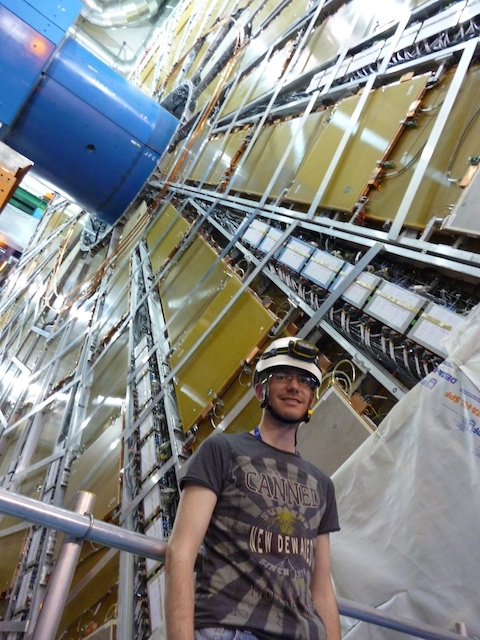
\includegraphics[width=0.48\textwidth]{tex/david_photo}
	\vspace{-20pt}
\end{wrapfigure}

David Hall obtained his DPhil degree at the University of Oxford whilst working on the ATLAS experiment at CERN. This research focussed on measuring the \WW production cross section and searching for evidence of the Higgs boson. Following this, David moved into proton therapy research and spent a short time at the Particle Therapy Cancer Research Institute, Oxford. He is now a postdoctoral research fellow at Massachusetts General Hospital and Harvard Medical School, developing Monte Carlo simulation programs and treatment planning systems for proton therapy. 

